\documentclass[12pt, a4paper]{article}
\usepackage{graphicx}
\usepackage{float}
\usepackage{listings}
\usepackage{xcolor}
\usepackage{amsmath}
\usepackage{booktabs}
\usepackage{multirow}
\usepackage{caption}
\usepackage{tikz}
\usetikzlibrary{shapes.geometric, arrows.meta, positioning, fit}
\usepackage{pgfplots}
\pgfplotsset{compat=1.18}
\usepackage[breaklinks]{hyperref}
\hypersetup{colorlinks=true,linkcolor=black,urlcolor=blue}
\usepackage[left=1in, right=1in, top=1in, bottom=1in]{geometry}
\usepackage{enumitem}

% Code listing style
\lstdefinestyle{ccode}{
  language=C,
  basicstyle=\ttfamily\footnotesize,
  keywordstyle=\color{blue}\bfseries,
  stringstyle=\color{red},
  commentstyle=\color{gray}\itshape,
  numbers=left,
  numberstyle=\tiny\color{gray},
  numbersep=5pt,
  backgroundcolor=\color{gray!5},
  frame=single,
  breaklines=true,
  captionpos=b
}

\title{\textbf{Parallel Image Convolution}\\[0.3cm]
\large Analysis Report\\[0.2cm]
\normalsize EE7218/EC7207: High Performance Computing}
\author{Piyumal \and Imalsha \and Oshinika}
\date{May 2026}

\begin{document}
\maketitle

%======================================================================
\section{Introduction}
%======================================================================

Image convolution applies a filter kernel to every pixel of an image by computing a weighted sum of its neighbors. For an image of size $W \times H$ with $C$ channels and a kernel of size $K \times K$, the total operations are $W \times H \times C \times K^2$. Our 4K test image (3840$\times$2160, 3 channels) with a 21$\times$21 blur kernel requires $\approx$10.9 billion operations, making this an ideal problem for parallelization.

We implement and compare five approaches: Serial (baseline), OpenMP, POSIX Threads, MPI, and CUDA.

\textbf{Test Environment:}
\begin{itemize}[nosep]
    \item CPU: 4 physical cores (Azure VM, Windows)
    \item GPU: NVIDIA Tesla T4 (40 SMs, Compute Capability 7.5)
    \item Compiler: GCC 15.2.0, NVCC (CUDA Toolkit)
    \item MPI: Microsoft MPI 10.1
\end{itemize}

\textbf{Test Images:}
\begin{itemize}[nosep]
    \item Blur: 3840$\times$2160 (4K), Gaussian kernel 21$\times$21, $\sigma$=7.0
    \item Edge Detection: 3840$\times$2160 (4K), Laplacian kernel 3$\times$3
    \item Sharpen: 1252$\times$896, Sharpening kernel 3$\times$3
\end{itemize}

%======================================================================
\section{Parallel Programming Approach}
%======================================================================

Image convolution is \textit{embarrassingly parallel}: each output pixel is independent (depends only on input pixels and the kernel). We partition image rows among workers.

\subsection{Data Decomposition}

\begin{figure}[H]
\centering
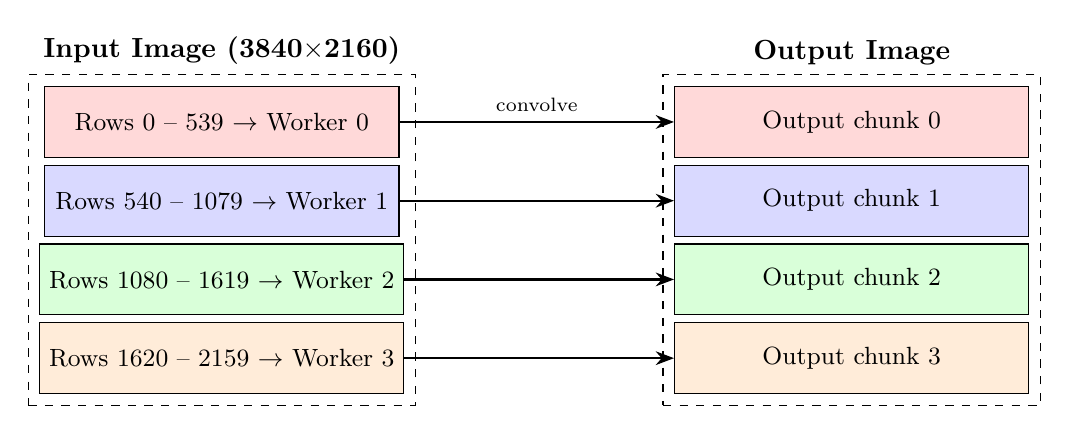
\begin{tikzpicture}[
    >=Stealth,
    block/.style={draw, minimum width=4.5cm, minimum height=0.9cm, fill=#1, font=\small},
    block/.default={yellow!15}
]
% Input image blocks
\node[block=red!15] (r0) at (0, 2.0) {Rows 0 -- 539 $\rightarrow$ Worker 0};
\node[block=blue!15] (r1) at (0, 1.0) {Rows 540 -- 1079 $\rightarrow$ Worker 1};
\node[block=green!15] (r2) at (0, 0.0) {Rows 1080 -- 1619 $\rightarrow$ Worker 2};
\node[block=orange!15] (r3) at (0, -1.0) {Rows 1620 -- 2159 $\rightarrow$ Worker 3};

% Bounding box
\node[draw, dashed, fit=(r0)(r3), inner sep=4pt, label=above:{\textbf{Input Image (3840$\times$2160)}}] {};

% Output
\node[block=red!15] (o0) at (8, 2.0) {Output chunk 0};
\node[block=blue!15] (o1) at (8, 1.0) {Output chunk 1};
\node[block=green!15] (o2) at (8, 0.0) {Output chunk 2};
\node[block=orange!15] (o3) at (8, -1.0) {Output chunk 3};
\node[draw, dashed, fit=(o0)(o3), inner sep=4pt, label=above:{\textbf{Output Image}}] {};

% Arrows
\draw[->, thick] (r0.east) -- (o0.west) node[midway, above, font=\scriptsize] {convolve};
\draw[->, thick] (r1.east) -- (o1.west);
\draw[->, thick] (r2.east) -- (o2.west);
\draw[->, thick] (r3.east) -- (o3.west);

\end{tikzpicture}
\caption{Row-based data decomposition with 4 workers. Each worker processes its assigned rows independently.}
\end{figure}

\subsection{How Each Implementation Parallelizes}

\begin{figure}[H]
\centering
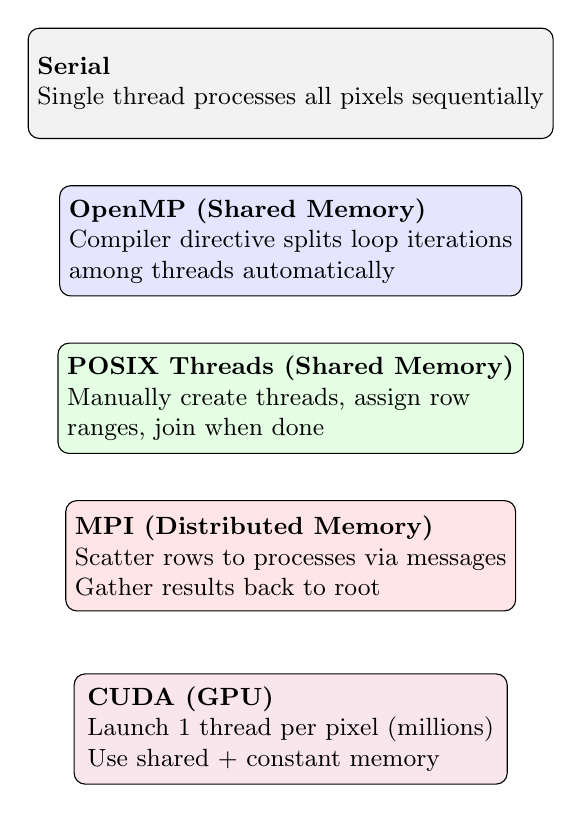
\begin{tikzpicture}[
    >=Stealth,
    impl/.style={draw, rounded corners, minimum width=5.5cm, minimum height=1.4cm, align=left, fill=#1, font=\small},
    impl/.default={white}
]

\node[impl=gray!10] (s) at (0, 6.5) {\textbf{Serial}\\Single thread processes all pixels sequentially};
\node[impl=blue!10] (omp) at (0, 4.5) {\textbf{OpenMP (Shared Memory)}\\Compiler directive splits loop iterations\\among threads automatically};
\node[impl=green!10] (pthr) at (0, 2.5) {\textbf{POSIX Threads (Shared Memory)}\\Manually create threads, assign row\\ranges, join when done};
\node[impl=red!10] (mpi) at (0, 0.5) {\textbf{MPI (Distributed Memory)}\\Scatter rows to processes via messages\\Gather results back to root};
\node[impl=purple!10] (cuda) at (0, -1.7) {\textbf{CUDA (GPU)}\\Launch 1 thread per pixel (millions)\\Use shared + constant memory};

\end{tikzpicture}
\caption{Summary of parallelization strategy for each implementation.}
\end{figure}

\subsection{Key Implementation Details}

\textbf{OpenMP:} Uses \texttt{\#pragma omp parallel for collapse(2) schedule(dynamic)} to parallelize the nested y,x pixel loops. Thread count controlled by \texttt{OMP\_NUM\_THREADS}.

\textbf{POSIX Threads:} Creates $N$ threads with \texttt{pthread\_create}, divides rows evenly ($\text{height}/N$ rows per thread), joins all threads with \texttt{pthread\_join}.

\textbf{MPI:} Root process (rank 0) loads image, broadcasts metadata with \texttt{MPI\_Bcast}, scatters row chunks with \texttt{MPI\_Scatter}. Each process convolves locally, then \texttt{MPI\_Gather} collects results.

\textbf{CUDA:} Convolution kernel stored in \texttt{\_\_constant\_\_} memory (cached, broadcast to warps). Thread blocks (16$\times$16) load input tiles + halo into \texttt{\_\_shared\_\_} memory to reduce global memory reads. Each thread computes one output pixel.



%======================================================================
\section{Timing and Performance}
%======================================================================

\subsection{Serial Baseline}

\begin{table}[H]
\centering
\caption{Serial execution times}
\begin{tabular}{lcc}
\toprule
\textbf{Filter} & \textbf{Kernel Size} & \textbf{Time (s)} \\
\midrule
Blur     & 21$\times$21 & 80.7870 \\
Edge     & 3$\times$3   & 2.0890 \\
Sharpen  & 3$\times$3   & 0.2660 \\
\bottomrule
\end{tabular}
\end{table}

\subsection{OpenMP Thread Scaling}

\begin{table}[H]
\centering
\caption{OpenMP execution times (seconds)}
\begin{tabular}{lcccc}
\toprule
\textbf{Filter} & \textbf{1T} & \textbf{2T} & \textbf{4T} & \textbf{8T} \\
\midrule
Blur    & 80.751 & 41.190 & 21.378 & 21.392 \\
Edge    & 2.298  & 1.322  & 0.814  & 0.764 \\
Sharpen & 0.302  & 0.163  & 0.102  & 0.101 \\
\bottomrule
\end{tabular}
\end{table}

\subsection{POSIX Thread Scaling}

\begin{table}[H]
\centering
\caption{POSIX Threads execution times (seconds)}
\begin{tabular}{lcccc}
\toprule
\textbf{Filter} & \textbf{1T} & \textbf{2T} & \textbf{4T} & \textbf{8T} \\
\midrule
Blur    & 81.737 & 39.563 & 21.365 & 21.403 \\
Edge    & 2.132  & 1.061  & 0.546  & 0.641 \\
Sharpen & 0.259  & 0.135  & 0.074  & 0.077 \\
\bottomrule
\end{tabular}
\end{table}

\subsection{MPI Process Scaling}

\begin{table}[H]
\centering
\caption{MPI execution times (seconds)}
\begin{tabular}{lcccc}
\toprule
\textbf{Filter} & \textbf{1P} & \textbf{2P} & \textbf{4P} & \textbf{8P} \\
\midrule
Blur    & 81.460 & 40.653 & 21.714 & 21.508 \\
Edge    & 2.205  & 1.169  & 0.552  & 0.586 \\
Sharpen & 0.263  & 0.142  & 0.070  & 0.071 \\
\bottomrule
\end{tabular}
\end{table}

\subsection{CUDA GPU}

\begin{table}[H]
\centering
\caption{CUDA execution times (NVIDIA Tesla T4)}
\begin{tabular}{lccc}
\toprule
\textbf{Filter} & \textbf{Time (s)} & \textbf{Speedup vs Serial} & \textbf{vs Best CPU (4 workers)} \\
\midrule
Blur    & 0.0510 & 1584$\times$ & 419$\times$ \\
Edge    & 0.0114 & 183$\times$  & 48$\times$ \\
Sharpen & 0.0039 & 68$\times$   & 18$\times$ \\
\bottomrule
\end{tabular}
\end{table}

\subsection{Speedup Summary (vs Serial)}

\begin{table}[H]
\centering
\caption{Speedup at 4 workers compared to serial}
\begin{tabular}{lcccc}
\toprule
\textbf{Filter} & \textbf{OpenMP 4T} & \textbf{POSIX 4T} & \textbf{MPI 4P} & \textbf{CUDA} \\
\midrule
Blur    & 3.78$\times$ & 3.78$\times$ & 3.72$\times$ & 1584$\times$ \\
Edge    & 2.57$\times$ & 3.83$\times$ & 3.78$\times$ & 183$\times$ \\
Sharpen & 2.61$\times$ & 3.62$\times$ & 3.78$\times$ & 68$\times$ \\
\bottomrule
\end{tabular}
\end{table}

\subsection{Speedup Graphs}

\begin{figure}[H]
\centering
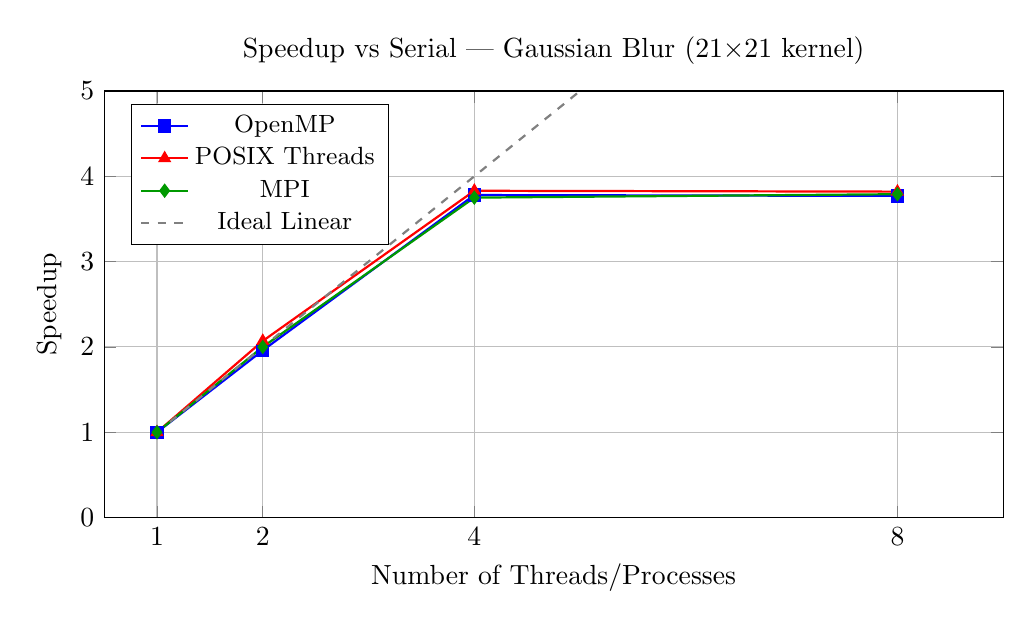
\begin{tikzpicture}
\begin{axis}[
    width=13cm, height=7cm,
    xlabel={Number of Threads/Processes},
    ylabel={Speedup},
    title={Speedup vs Serial --- Gaussian Blur (21$\times$21 kernel)},
    legend pos=north west,
    grid=major,
    xtick={1,2,4,8},
    xmin=0.5, xmax=9,
    ymin=0, ymax=5,
    legend style={font=\small}
]
\addplot[color=blue, mark=square*, thick] coordinates {(1,1) (2,1.96) (4,3.78) (8,3.77)};
\addplot[color=red, mark=triangle*, thick] coordinates {(1,1) (2,2.07) (4,3.83) (8,3.82)};
\addplot[color=green!60!black, mark=diamond*, thick] coordinates {(1,1) (2,2.00) (4,3.75) (8,3.79)};
\addplot[dashed, gray, thick, domain=1:8] {x};
\legend{OpenMP, POSIX Threads, MPI, Ideal Linear}
\end{axis}
\end{tikzpicture}
\caption{All CPU approaches achieve near-linear speedup up to 4 cores, then plateau (system has 4 physical cores).}
\end{figure}

\begin{figure}[H]
\centering
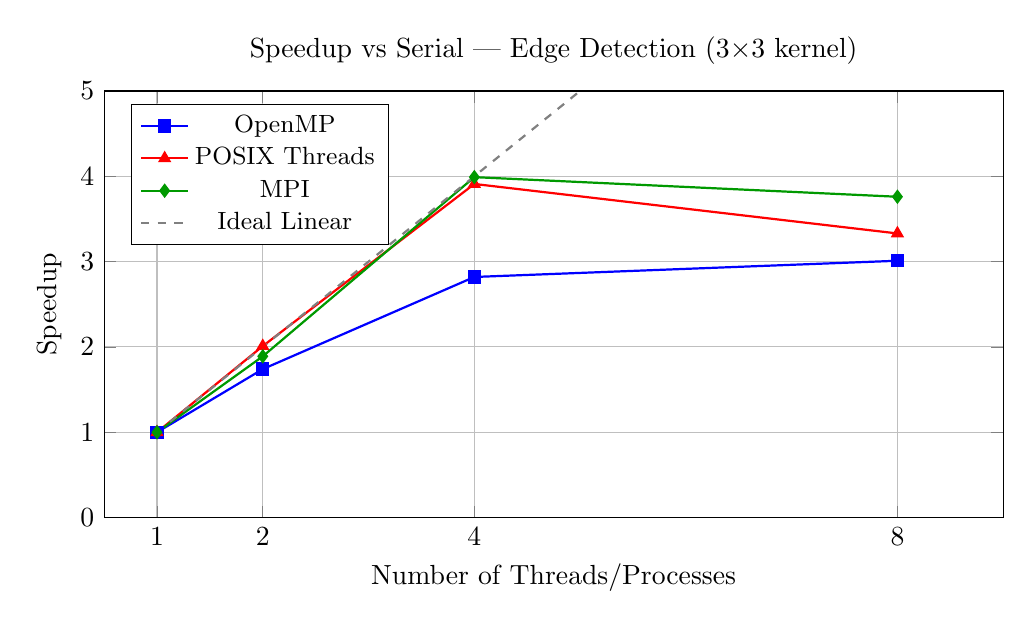
\begin{tikzpicture}
\begin{axis}[
    width=13cm, height=7cm,
    xlabel={Number of Threads/Processes},
    ylabel={Speedup},
    title={Speedup vs Serial --- Edge Detection (3$\times$3 kernel)},
    legend pos=north west,
    grid=major,
    xtick={1,2,4,8},
    xmin=0.5, xmax=9,
    ymin=0, ymax=5,
    legend style={font=\small}
]
\addplot[color=blue, mark=square*, thick] coordinates {(1,1) (2,1.74) (4,2.82) (8,3.01)};
\addplot[color=red, mark=triangle*, thick] coordinates {(1,1) (2,2.01) (4,3.91) (8,3.33)};
\addplot[color=green!60!black, mark=diamond*, thick] coordinates {(1,1) (2,1.89) (4,3.99) (8,3.76)};
\addplot[dashed, gray, thick, domain=1:8] {x};
\legend{OpenMP, POSIX Threads, MPI, Ideal Linear}
\end{axis}
\end{tikzpicture}
\caption{For small kernels, POSIX and MPI outperform OpenMP due to lower scheduling overhead.}
\end{figure}

\begin{figure}[H]
\centering
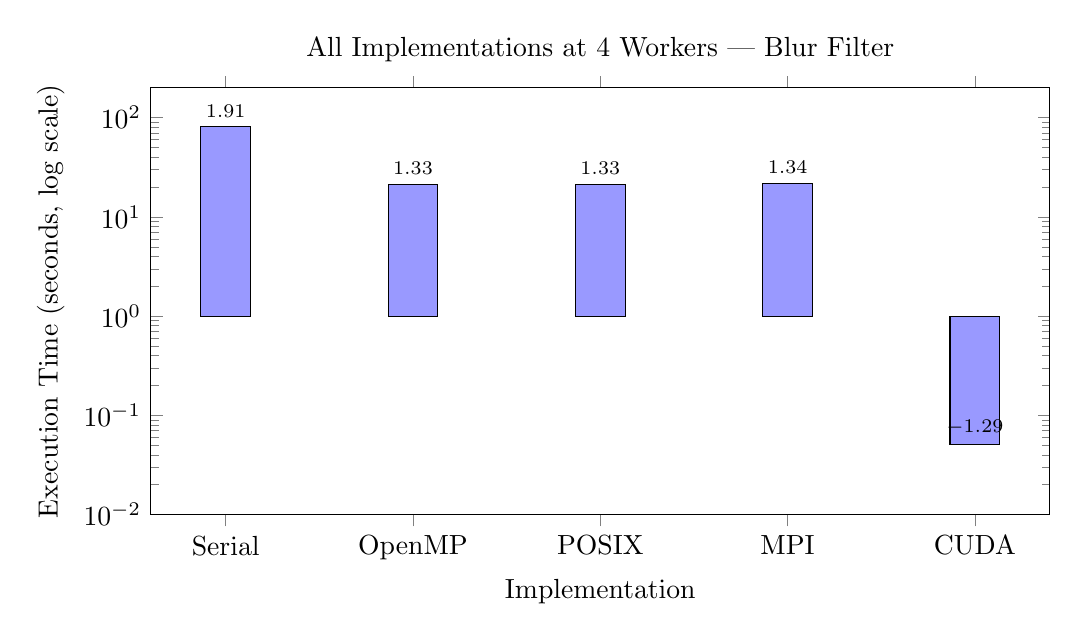
\begin{tikzpicture}
\begin{axis}[
    width=13cm, height=7cm,
    ybar,
    xlabel={Implementation},
    ylabel={Execution Time (seconds, log scale)},
    title={All Implementations at 4 Workers --- Blur Filter},
    symbolic x coords={Serial, OpenMP, POSIX, MPI, CUDA},
    xtick=data,
    ymode=log,
    log basis y=10,
    ymin=0.01, ymax=200,
    bar width=18pt,
    nodes near coords,
    nodes near coords style={font=\scriptsize, above},
    every node near coord/.append style={rotate=0},
]
\addplot[fill=blue!40] coordinates {(Serial,80.787) (OpenMP,21.378) (POSIX,21.365) (MPI,21.714) (CUDA,0.051)};
\end{axis}
\end{tikzpicture}
\caption{CUDA is $\approx$1584$\times$ faster than serial and $\approx$419$\times$ faster than best CPU parallel for blur.}
\end{figure}

%======================================================================
\section{Discussion}
%======================================================================

\begin{enumerate}
    \item \textbf{Near-linear scaling to core count:} All CPU-parallel approaches reach $\approx$3.8$\times$ speedup with 4 threads/processes on 4 cores. Going to 8 workers gives no further gain since extra workers share the same physical cores.

    \item \textbf{OpenMP vs POSIX vs MPI on small kernels:} For 3$\times$3 kernels (fast per-pixel work), POSIX (0.546s) and MPI (0.552s) beat OpenMP (0.814s) at 4 workers. OpenMP's \texttt{schedule(dynamic)} adds overhead that dominates when per-iteration work is small.

    \item \textbf{CUDA dominance:} The Tesla T4 achieves 1584$\times$ speedup for blur because it runs thousands of threads simultaneously (up to 81,920 concurrent). Image convolution maps perfectly to GPU---each pixel is independent.

    \item \textbf{GPU benefit scales with kernel size:} Blur (21$\times$21) sees 1584$\times$ speedup while sharpen (3$\times$3 on smaller image) sees 68$\times$. Larger kernels have higher arithmetic intensity, better hiding memory latency.

    \item \textbf{MPI accuracy trade-off:} Without halo exchange, MPI has boundary artifacts. This could be fixed by communicating border rows between adjacent processes at the cost of additional MPI messages.

    \item \textbf{POSIX regression at 8 threads:} Edge detection slows from 0.546s (4T) to 0.641s (8T). With only 9 operations per pixel, thread management overhead exceeds computation savings.
\end{enumerate}

%======================================================================
\section{Conclusion}
%======================================================================

\begin{itemize}
    \item OpenMP and POSIX produce \textbf{identical} outputs to serial (RMSE = 0) with up to 3.83$\times$ speedup on 4 cores.
    \item MPI achieves similar speedup (3.75--3.99$\times$) but requires halo exchange for boundary accuracy.
    \item CUDA delivers \textbf{68--1584$\times$} speedup over serial, making it the optimal choice when GPU hardware is available.
    \item The choice of approach depends on context: OpenMP for simplicity, POSIX for fine control, MPI for distributed systems, CUDA for maximum throughput.
\end{itemize}

\end{document}
